\begin{slide}{Object Manipulation}
  Two types of objects
  \begin{itemize}
  \item $C \rightarrow$ objects to be collected
  \item $D \rightarrow$ objects to be destroyed
  \end{itemize}
  Swarm Goal
  \begin{itemize}
  \item Collect all $C$ objects
  \item Destroy all $D$ objects
  \end{itemize}
  Approach
  \begin{enumerate}
  \item Collection
  \item Destruction
  \item \fbox{Collection and Destruction}
  \end{enumerate}
\end{slide}

%%%%%
%%%%%

\begin{slide}{Object Manipulation} 
  \centering
  \tiny
  \begin{tabular}{|l||c|c|c|}
    \hline
    \multirow{2}{*}{\textbf{Behavior}} & \multicolumn{3}{c|}{\textbf{Scenarios}}  \\
    & Collection & Destruction & Manipulation \\	
    \hline
    \emph{move-up}           & x & x & x \\
    \emph{move-down}         & x & x & x \\
    \emph{move-left}         & x & x & x \\
    \emph{move-right}        & x & x & x \\
    \emph{move-random}       & x & x & x \\
    \emph{pick-up}           & x &   & x \\
    \emph{put-down}          & x &   & x \\
    \emph{move-to-goal}      & x &   & x \\
    \emph{broadcast\_C}      & x &   & x \\
    \emph{move-to-object\_C} & x &   & x \\
    \emph{first-attack}      &   & x & x \\
    \emph{second-attack}     &   & x & x \\
    \emph{broadcast\_D}      &   & x & x \\ 
    \emph{move-to-object\_D} &   & x & x \\
    \hline
  \end{tabular}
\end{slide}

%%%%%
%%%%%

\begin{slide}{Object Manipulation}
  \centering
  \tiny
  \begin{tabular}{|l||c|c|c|}
    \hline
    \multirow{2}{*}{\textbf{Sensor}} & \multicolumn{3}{c|}{\textbf{Scenarios}}  \\
    & Collection & Destruction & Manipulation \\
    \hline
    \hline
    \emph{near-object\_C}          & x &   & x \\
    \emph{on-object\_C}            & x &   & x \\
    \emph{holding-object\_C}       & x &   & x \\
    \emph{on-goal}                 & x &   & x \\
    \hline
    \emph{near-object\_D}          &   & x & x \\
    \emph{on-object\_D(untouched)} &   & x & x \\
    \emph{on-object\_D(damaged)}   &   & x & x \\
    \hline
  \end{tabular}
\end{slide}

%%%%%
%%%%%

\begin{slide}{Object Manipulation}
  \centering
  \tiny
  \bigskip
  \begin{tabular}{c|l}
    Fitness Metric & Description \\
    \hline
    $c_{1}$ & number of objects picked up but not put in the goal   \\
    $c_{2}$ & number of objects not collected \\
    $d_{1}$ &  number of objects in the partially destroyed state  \\
    $d_{2}$ &  number of objects in the untouched state \\
    $t$         &  number of time steps \\
  \end{tabular}
\end{slide}

%%%%%
%%%%%

\begin{slide}{Object Manipulation}
  The challenge 
  \vspace{3ex}
  \begin{center}
    \begin{quote}
      \centering
      \em Collection and destruction metrics \\
      are independent but equally weighted
    \end{quote}
  \end{center}
  \vspace{2ex}
  \begin{itemize}
  \item Imposing an order skews evolution
  \item ``Experts'' are evolved
  \item Solution
    \begin{itemize}
    \item Construct new composite metrics
    \item Eliminate sequential dependencies
    \item Rank solutions using radix-based sorting
    \end{itemize}
  \end{itemize}
\end{slide}

%%%%%
%%%%%

\begin{slide}{Object Manipulation}
  \centering
  \bigskip
  \begin{tabular}{c|c|l}
    Composite Metric & Composition & Description \\
    \hline
    $m_1$ & $\sim c_1 \wedge \sim d_1$ & flag, fully performing both \\
    $m_2$ & $\sim c_2 \wedge \sim d_2$ & flag, partially performing both \\
    $m_3$ & $\sim c_1 \vee \sim d_1$   & flag, fully performing either \\
    $m_4$ & $\sim c_2 \vee \sim d_2$   & flag, partially performing either \\
    $m_5$ & $\max(c_1,d_1)$ & select the weakest \\
    $m_6$ & $\max(c_2,d_2)$ & select the weakest \\
    $m_7$ & $\min(c_1,d_1)$ & select the strongest \\
    $m_8$ & $\min(c_2,d_2)$ & select the strongest \\
    $m_9$ & $t$ & number of timesteps \\
  \end{tabular}
\end{slide}

%%%%%
%%%%%

\begin{slide}{Object Manipulation}
  Parameters
  \begin{itemize}
  \item Population: 32
  \item Mutations: all top 6 + 2 random
  \item \SWEEP: 100 agents, $50\times50$ grid
  \item $C$ objects = 50
  \item $D$ objects = 30
  \item Broadcast range = 25
  \item Sensing range = 5
  \end{itemize}
\end{slide}

%%%%%
%%%%%

\begin{slide}{Object Manipulation}
  Results Summary
\end{slide}

%%%%%
%%%%%

\overlays{2}{%
  \begin{slide}{Object Manipulation}
    \onlySlide*{1}{%
      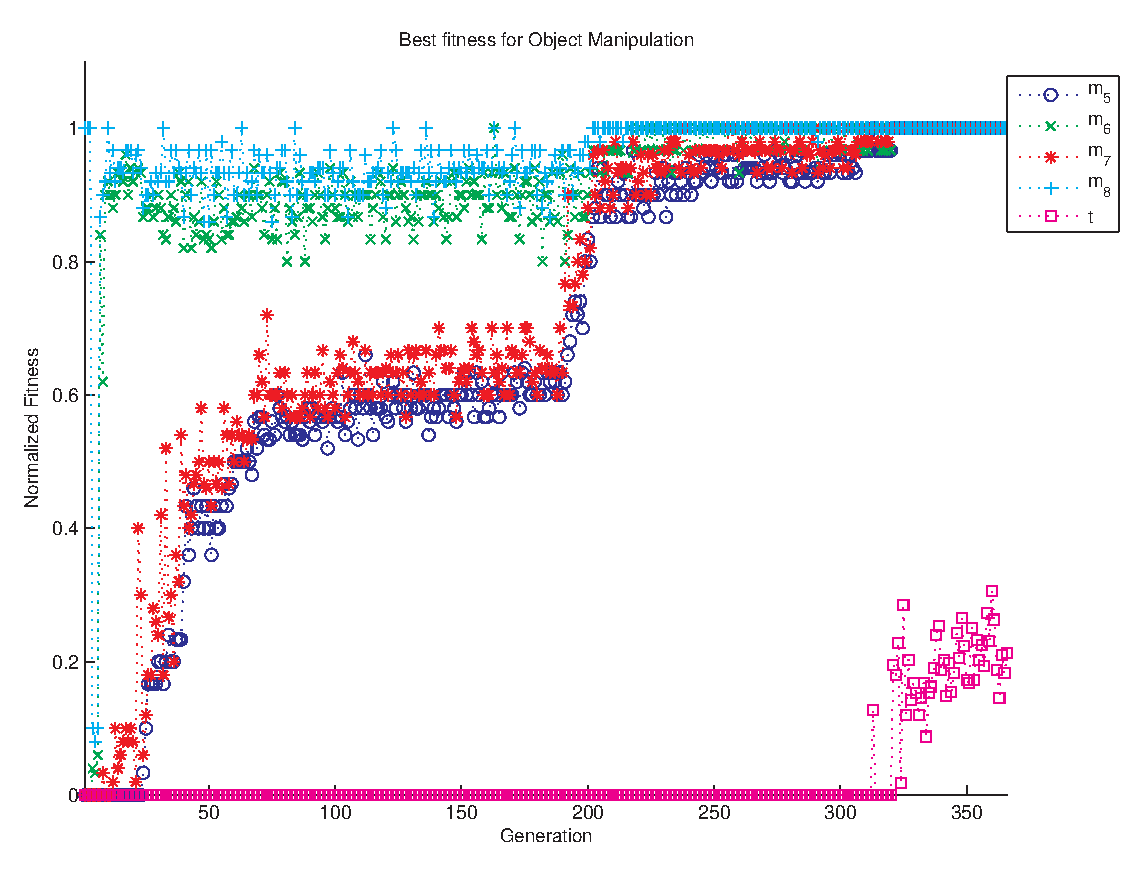
\includegraphics[height=\textheight]{ObjectManipulationBest-1}
    }%
    
    \onlySlide*{2}{%
      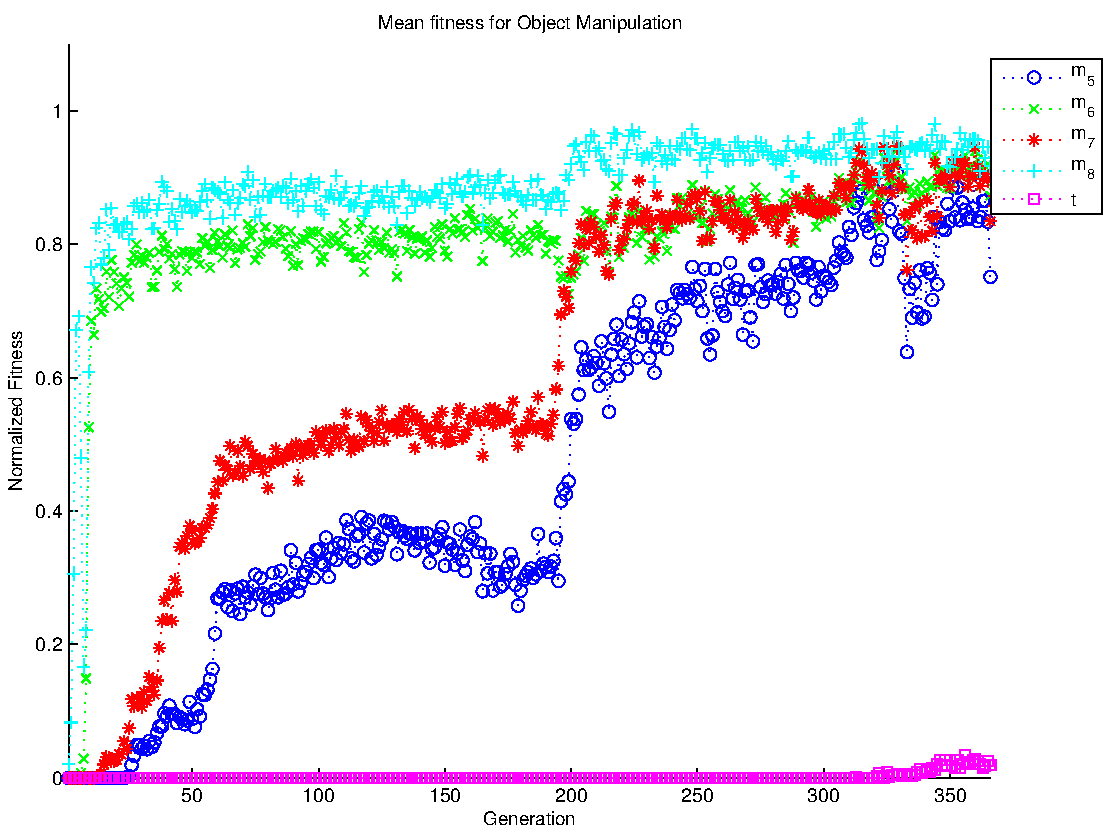
\includegraphics[height=\textheight]{ObjectManipulationMean-1}
    }%
  \end{slide}
}%

%%%%%
%%%%%

\overlays{2}{%
  \begin{slide}{Object Manipulation}
    \centering
    \onlySlide*{1}{%
      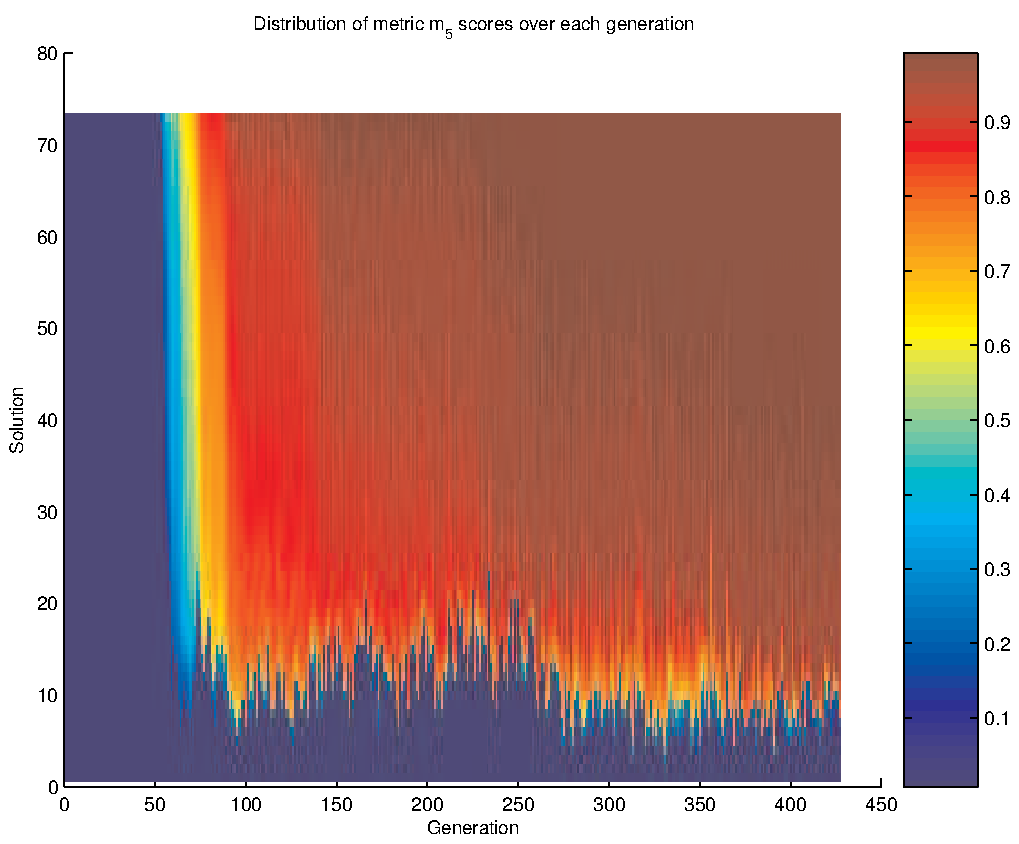
\includegraphics[height=\textheight]{ObjectManipulationM5-2}
    }%
    
    \onlySlide*{2}{%
      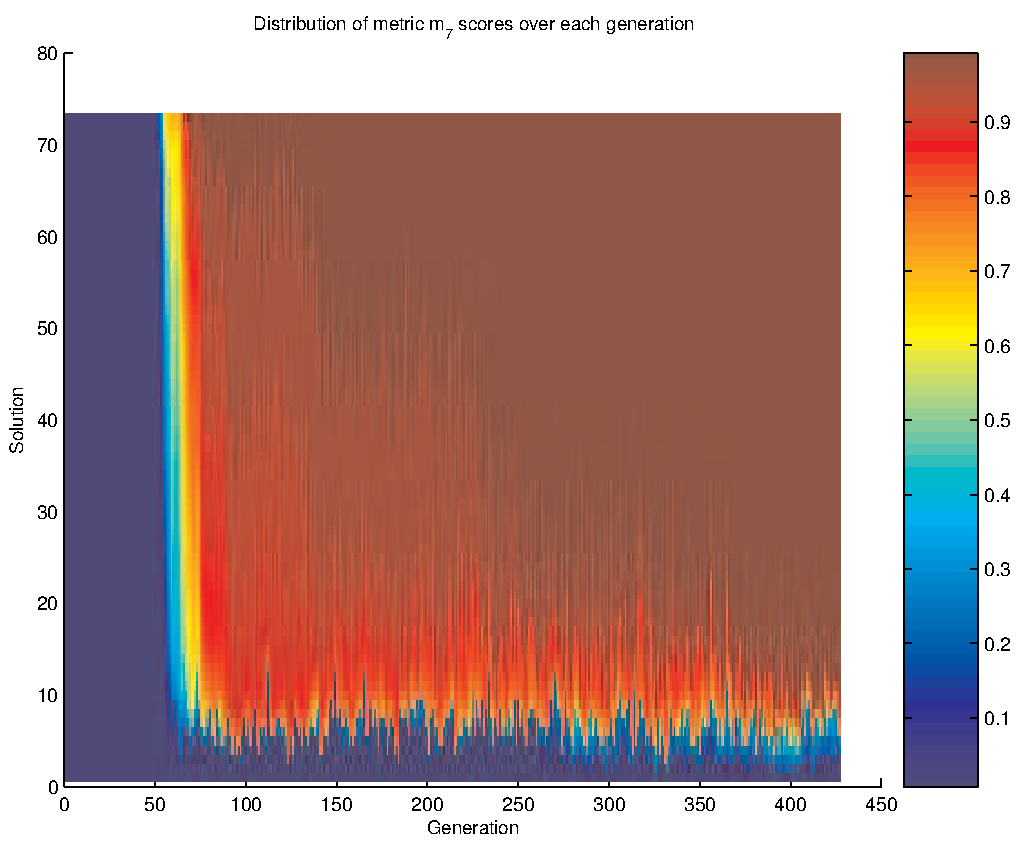
\includegraphics[height=\textheight]{ObjectManipulationM7-2}
    }%
  \end{slide}
}%

